%!TEX root=../GaugeCNNTheory.tex


\subsection{\lr{CNN}های کروی هموردای دوران سمتی در توپولوژی‌های استوانه‌ای}
\label{sec:spherical_CNNs_azimuthal_equivariant}



علاوه بر کانولوشن‌های کروی کاملاً $\SO3$- یا $\O3$-هموردا، بسیاری از \lr{CNN}های کروی طوری طراحی شده‌اند که نسبت به دوران‌های سمتی حول یک محور قطبی مشخص، هموردا باشند.
تمام مدل‌های مورد بحث در این بخش یا بر $\SO2$-ساختار $\{e\}$-ناوردا که در شکل‌های~\ref{fig:G_structure_S2_2} و \ref{fig:spherical_equirectangular_1} نشان داده شده است، یا به طور جایگزین، بر ساختار نشان داده شده در شکل~\ref{fig:spherical_equirectangular_2} تکیه دارند.
به دلیل بدیهی بودن گروه ساختار $G=\{e\}$، فضاهای کرنل نامحدود باقی می‌مانند ($\{e\}$-راهبری‌پذیر).
ویژگی‌ها مطابق با اتصال بدیهی یکتای $\{e\}$-سازگار منتقل می‌شوند که با اتصال لوی-چیویتا کروی معمول متفاوت است.
با این اطلاعات، و با نگاشت‌های نمایی صریح در معادله~\eqref{eq:sphere_expmap_explicit}، کانولوشن‌های $\GM$ کروی در این بخش در تئوری کاملاً مشخص شده‌اند.
در عمل، پیاده‌سازی‌ها، که در ردیف (۳۴) جدول~\ref{tab:network_instantiations} فهرست شده‌اند، در پیاده‌سازی‌های عددی خود متفاوت هستند، که در ادامه به بحث در مورد آنها می‌پردازیم.


\begin{SCfigure}
    \centering
    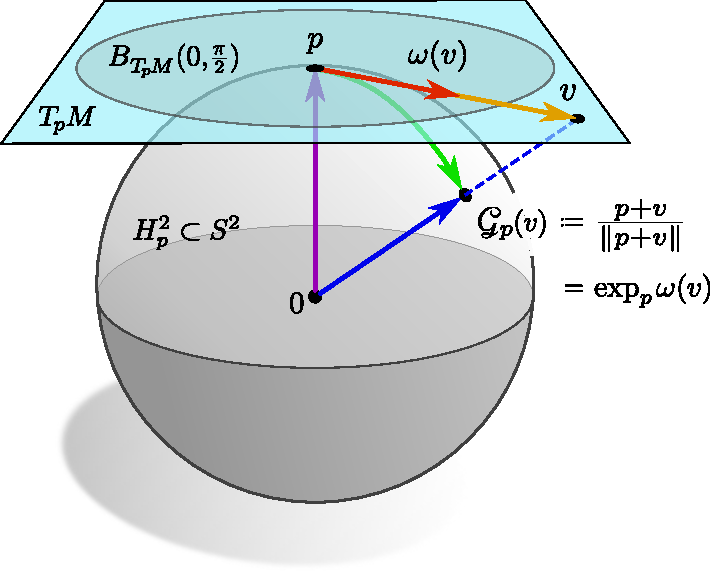
\includegraphics[width=.55\textwidth]{figures/gnomonic_proj.pdf}
    \captionsetup{width=1.02\textwidth}
    \hspace{1ex}
    \caption{\small
        تصویر نومونیک ${\mathscr{G}_p\!: \TpM \to H_p^2}$ از فضای مماس در $p$ به نیمکره بالایی $H_p^2 \subset S^2$ حول~$p$.
        هنگامی که کره به عنوان جایگذاری شده در $\R^3$ تفسیر شود، تصویر نومونیک $\mathscr{G}_p(v)$ (آبی) با مجموع ${p\in S^2 \subset \R^3}$ (بنفش) و $v\in\TpM \subset\R^3$ (زرد) در فضای محیطی، و به دنبال آن یک نرمال‌سازی برای بازگشت به کره، داده می‌شود.
        قضیه~\ref{thm:gnomonic} اثبات می‌کند که این عملیات معادل یک تصویر از یک بردار با تاب شعاعی $\omega(v) = \arctan(\lVert v\rVert) \frac{v}{\lVert v\rVert} \in B_{\TpM}(0,{\textstyle\frac{\pi}{2}})$ (قرمز) از طریق نگاشت نمایی (سبز) است.
        بنابراین، کانولوشن‌های کروی مبتنی بر تصویر نومونیک در
        \cite{coors2018spherenet,zhao2018distortion,tateno2018distortion,eder2019convolutions,martin2020panoramic}
        موارد خاصی از کانولوشن‌های $\GM$ کروی با کرنل‌های دارای تاب شعاعی هستند.
        کانولوشن‌های $\GM$ عمومی‌تر هستند زیرا به تصویرهای کرنل روی کل کره به جای فقط نیمکره بالایی اجازه می‌دهند.
        \\\protect\rule{0ex}{0.ex}
    }
    \label{fig:gnomonic_proj}
\end{SCfigure}


همزمان با تعریف ما از اشتراک وزن کانولوشنی، مدل‌های \cite{coors2018spherenet,zhao2018distortion,tateno2018distortion,eder2019convolutions,martin2020panoramic} یک کرنل الگوی داده شده را روی فضاهای مماس با جهت‌دهی آن نسبت به چارچوب‌های $\{e\}$-ساختار در نظر گرفته شده در شکل~\ref{fig:G_structure_S2_2} به اشتراک می‌گذارند.
با این حال، برخلاف کانولوشن‌های $\GM$, تطبیق این کرنل‌ها با میدان ویژگی از طریق نگاشت‌های نمایی (یا پول‌بک‌های انتقال‌دهنده) انجام نمی‌شود، بلکه از طریق تصویر نومونیک انجام می‌شود.
این تصویر نومونیک در هر نقطه $p$ با
\begin{align}\label{eq:gnomonic_proj_def}
    \mathscr{G}_p:\, \TpM \to H_p^2, \quad v \mapsto \frac{p+v}{\lVert p+v\rVert} \,,
\end{align}
تعریف می‌شود، که در شکل~\ref{fig:gnomonic_proj} به تصویر کشیده شده است.
جمع $p\in S^2 \subset \R^3$ با بردارهای مماس $v \in \TpM \subset \R^3$ در اینجا در فضای جایگذاری $\R^3$ انجام می‌شود و نرمال‌سازی نتیجه را به کره باز می‌گرداند.
هم‌دامنه تصویر نومونیک، نیمکره «بالایی»
\begin{align}\label{eq:upper_hemisphere_def}
    H_p^2 := \big\{ q\in S^2 \,\big|\, \langle p,q\rangle_{\R^3} > 0 \big\} \,\subset S^2
\end{align}
است که حول $p$ متمرکز شده است.
با توجه به این تفاوت در تصویرهای کرنل، ممکن است به نظر برسد که مدل‌های \cite{coors2018spherenet,zhao2018distortion,tateno2018distortion,eder2019convolutions,martin2020panoramic} به عنوان کانولوشن $\GM$ توضیح داده نمی‌شوند (یا فقط به طور تقریبی).
قضیه زیر، با این حال، اثبات می‌کند که تصویر نومونیک معادل یک تصویر از طریق نگاشت نمایی پس از اعمال یک \emph{تاب شعاعی}
\begin{align}\label{eq:radial_warp}
    \omega:\ \TpM \to B_{\TpM}(0,{\textstyle\frac{\pi}{2}}), \quad
    v \mapsto \arctan\! \big(\lVert v\rVert\big) \frac{v}{\lVert v\rVert}
\end{align}
به فضاهای مماس است، که بردارهای مماس را به یک گوی باز با شعاع $\pi/2$ حول مبدأ منقبض می‌کند:
\begin{thm}[تصویرهای نومونیک به عنوان نگاشت‌های نمایی دارای تاب]
\label{thm:gnomonic}
    تصویر نومونیک $\mathscr{G}_p$ از $\TpM$ به نیمکره بالایی $H_p^2\subset S^2$ که در معادله~\eqref{eq:gnomonic_proj_def} تعریف شده است، معادل یک تصویر از تاب شعاعی آن $\omega(\TpM) = B_{\TpM}(0,{\textstyle\frac{\pi}{2}})$ (معادله~\eqref{eq:radial_warp}) از طریق نگاشت نمایی است، یعنی نمودار زیر جابجایی است:
    \begin{equation}\label{cd:gnomonic_exp_warp}
    \begin{tikzcd}[column sep=60, row sep=6pt, font=\normalsize]
        \TpM
            \arrow[dr, pos=.45, "\mathscr{G}_p"]
            \arrow[dd, "\omega\,"']
        \\
        & H_p^2 \subset S^2
        \\
        B_{\TpM}(0,{\textstyle\frac{\pi}{2}})
            \arrow[ur, pos=.3, "\exp_p"']
    \end{tikzcd}
    \end{equation}
    در معادلات،
    \begin{align}
        \mathscr{G}_p(v) \,=\, \exp_p \circ\, \omega(v)
    \end{align}
    برای هر $p\in S^2$ و هر $v\in\TpM$ برقرار است.
\end{thm}
\begin{proof}
    اثبات با محاسبه ساده زیر داده می‌شود، که برای هر $p\in S^2$ و هر $v\in \TpM$ برقرار است:
    \begin{align}
        \exp_p \circ\mkern2mu \omega (v)
        \ &\overset{(1)}{=}\ p\cdot \cos\! \big(\lVert \omega(v)\rVert\big) \,+\, \frac{\omega(v)}{\lVert \omega(v)\rVert}\cdot \sin\! \big(\lVert \omega(v)\rVert\big) \notag \\
        \ &\overset{(2)}{=}\ p\cdot \cos\! \big(\!\arctan(\lVert v\rVert)\big) \,+\, \frac{v}{\lVert v\rVert}\cdot \sin\! \big(\!\arctan(\lVert v\rVert)\big) \notag \\
        \ &\overset{(3)}{=}\ \frac{p+v}{\sqrt{1+\lVert v\rVert^2}} \notag \\
        \ &\overset{(4)}{=}\ \frac{p+v}{\lVert p+v\rVert} \notag \\
        \ &\overset{(5)}{=}\ \mathscr{G}_p(v)
    \end{align}
    مراحل اول و دوم از تعریف صریح نگاشت نمایی کره جایگذاری شده، معادله~\eqref{eq:sphere_expmap_explicit}، و تاب شعاعی، معادله~\eqref{eq:radial_warp}، استفاده می‌کنند.
    مرحله سوم از آنجا نتیجه می‌شود که $\cos \circ \arctan(x) = \frac{1}{\sqrt{1+x^2}}$ و $\sin \circ \arctan(x) = \frac{x}{\sqrt{1+x^2}}$.
    در مرحله چهارم ما از این استفاده کردیم که $\lVert p\rVert = 1$ و $\langle p,v\rangle_{\R^3} = 0$, در حالی که مرحله آخر تصویر نومونیک، معادله~\eqref{eq:gnomonic_proj_def} را شناسایی کرد.
\end{proof}
این قضیه دلالت بر این دارد که کانولوشن‌های مبتنی بر تصویر نومونیک در
\cite{coors2018spherenet,zhao2018distortion,tateno2018distortion,eder2019convolutions,martin2020panoramic}
در واقع موارد خاصی از کانولوشن‌های $\GM$ پس از یکی گرفتن کرنل‌ها از طریق تاب شعاعی $\omega$ هستند.%
\footnote{
    از نظر فنی، معادل بودن هر دو کانولوشن علاوه بر این نیازمند یک تغییر وابسته به شعاع در دامنه کرنل برای در نظر گرفتن تغییر در اندازه حجم هنگام تاب دادن کرنل است.
}
توجه داشته باشید که این یکی گرفتن نه تنها برای کرنل‌های $\{e\}$-راهبری‌پذیر بلکه برای هر زیرگروه $G\leq\O2$ نیز برقرار است زیرا محدودیت‌های $G$-راهبری‌پذیری متناظر فقط بر بخش‌های زاویه‌ای کرنل‌ها تأثیر می‌گذارند اما مستقل از بخش‌های شعاعی تاب‌داده شده هستند.
ما علاوه بر این می‌خواهیم اشاره کنیم که تصویر مبتنی بر نگاشت نمایی در کانولوشن‌های $\GM$ از این جهت عمومی‌تر از تصویر کرنل نومونیک است که می‌تواند کرنل‌هایی را توصیف کند که فراتر از نیمکره بالایی $H_p^2$ حول~$p$ گسترش می‌یابند.
توجه داشته باشید که هر دو تصویر کرنل در حد عملی مرتبط کرنل‌های کوچک، حتی بدون تاب شعاعی، معادل می‌شوند زیرا $\arctan\big(\lVert v\rVert\big) = \lVert v\rVert + \mathcal{O}\big(\lVert v\rVert^3\big)$.

پیاده‌سازی‌های \cite{coors2018spherenet,zhao2018distortion,tateno2018distortion,eder2019convolutions,martin2020panoramic}
در پیوستار همگی با یکدیگر و با کانولوشن $\GM$ ما معادل هستند، با این حال، گسسته‌سازی‌های عددی آنها متفاوت است.
\citet{coors2018spherenet}، \citet{eder2019convolutions} و \citet{martin2020panoramic} میدان‌های ویژگی را روی شبکه‌های نمونه‌برداری (تقریباً) یکنواخت روی کره گسسته‌سازی می‌کنند.
به طور خاص، \citet{coors2018spherenet} و \citet{martin2020panoramic} از «مجموعه مارپیچ تعمیم‌یافته روی~$S^2$» از~\cite{saff1997distributing} به عنوان نقاط نمونه‌برداری استفاده می‌کنند، در حالی که \citet{eder2019convolutions} از رئوس یک ایکوسفر استفاده می‌کنند.
از آنجا که تصویرهای نومونیک از شبکه‌های نمونه‌برداری کرنل روی فضاهای مماس با شبکه نمونه‌برداری کروی مطابقت ندارند، نویسندگان بین آنها درون‌یابی دوخطی انجام می‌دهند.
ضرایب نمونه‌برداری کرنل در اینجا می‌توانند در یک مرحله آفلاین از پیش محاسبه شوند.
کانولوشن واقعی سپس یک میدان ویژگی خروجی را با منقبض کردن کرنل‌های تصویر شده و درون‌یابی شده در هر نقطه با میدان ورودی محاسبه می‌کند.


\begin{figure}
    \centering
    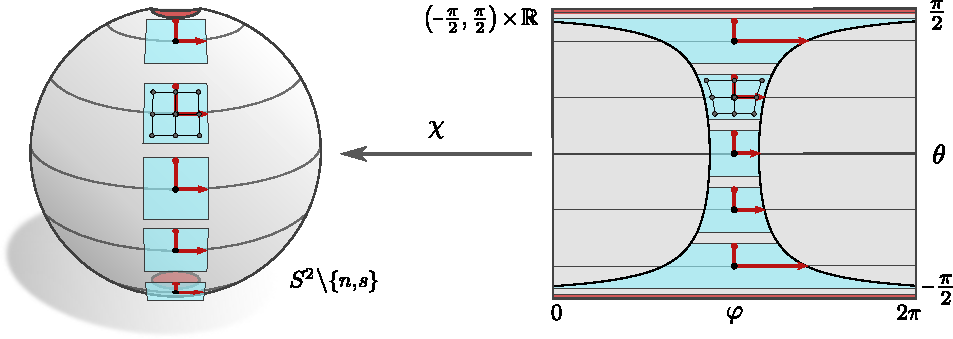
\includegraphics[width=.90\textwidth]{figures/G_structure_spherical_equirectangular_1.pdf}
    \caption{\small
        نمایش $\{e\}$-ساختار $\SO2$-ناوردا که توسط اکثر مدل‌های مورد بحث در بخش~\ref{sec:spherical_CNNs_azimuthal_equivariant} در نظر گرفته شده است.
        تمام چارچوب‌ها
        $\big[ \frac{\partial}{\partial\theta} ,\; \frac{1}{\cos(\theta)} \frac{\partial}{\partial\varphi} \big]$
        به سمت قطب شمال تراز شده‌اند و نسبت به متریک جایگذاری کره در $\R^3$ راست‌هنجار هستند.
        نگاشت مختصات کروی
        $\chi: (-\frac{\pi}{2}, \frac{\pi}{2}) \times \R \to S^2 \backslash \{n,s\}$ از معادله~\eqref{eq:spherical_coords}
        اجازه می‌دهد تا میدان‌های ویژگی کروی به میدان‌های ویژگی روی زوایای کروی $(-\frac{\pi}{2}, \frac{\pi}{2}) \times \R$ پول‌بک شوند، که به آن تصویر هم‌مستطیلی (equirectangular) گفته می‌شود.
        از آنجا که~$\chi$ ایزومتریک نیست، $\{e\}$-ساختار کروی در مختصات با یک ضریب وابسته به عرض جغرافیایی $1/\cos(\theta)$ که به سمت قطب‌ها واگرا می‌شود، تغییر شکل می‌یابد.
        کانولوشن کروی روی این $\{e\}$-ساختار در~\cite{coors2018spherenet,eder2019convolutions,martin2020panoramic} با تصویر کردن و درون‌یابی یک شبکه نمونه‌برداری کرنل روی فضاهای مماس به یک شبکه نمونه‌برداری میدان ویژگی روی کره پیاده‌سازی می‌شود.
        اگر میدان‌های ویژگی در عوض روی تصویر هم‌مستطیلی نمونه‌برداری شوند، شبکه نمونه‌برداری کرنل در مرحله دوم از کره به یک شبکه نمونه‌برداری تغییر شکل یافته روی $(-\frac{\pi}{2}, \frac{\pi}{2}) \times \R$ نگاشت داده می‌شود \cite{zhao2018distortion,tateno2018distortion}.
        توجه داشته باشید که شبکه‌های نمونه‌برداری منظم روی تصویر هم‌مستطیلی سیگنال را (نسبت به متریک کروی) به سمت قطب‌ها بیش‌نمونه‌برداری می‌کنند.
    }
    \label{fig:spherical_equirectangular_1}
\end{figure}


\citet{zhao2018distortion} و \citet{tateno2018distortion} میدان‌های ویژگی کروی خود $f: S^2 \backslash \{n,s\} \to \R^c$ را در عوض به شکل یک شبکه پیکسلی منظم روی یک تصویر هم‌مستطیلی از کره گسسته‌سازی می‌کنند.
از نظر ریاضی، تصویر هم‌مستطیلی، که در شکل~\ref{fig:spherical_equirectangular_1} به تصویر کشیده شده است، به عنوان پول‌بک
$\chi^*f = f \circ \chi: \big(\minus\frac{\pi}{2}, \frac{\pi}{2}\big) \times \R \to \R^c$
از تصویر توسط نگاشت مختصات کروی $\chi$ از معادله~\eqref{eq:spherical_coords} رسمیت می‌یابد:
\begin{equation}\label{cd:equirectangular_proj}
\begin{tikzcd}[column sep=50pt, row sep=25pt, font=\normalsize]
    {\big(\minus\frac{\pi}{2}, \frac{\pi}{2}\big)} \times \R
        \arrow[r, "\chi"]
        \arrow[rr, pos=.5, rounded corners, to path={ 
            -- ([yshift=-2.5ex]\tikztostart.south) 
            --node[below]{\small$
                \chi^*f
                $} ([yshift=-2.5ex]\tikztotarget.south) 
            -- (\tikztotarget.south)
            }]
    & S^2 \backslash \{n,s\}
        \arrow[r, "f"]
    & \R^c \mkern-12mu\phantom{\big)}
\end{tikzcd}
\end{equation}
همانند رویکردهای قبلی، نویسندگان یک شبکه نمونه‌برداری کرنل را از طریق تصویر نومونیک از فضاهای مماس به کره تصویر می‌کنند.
در یک مرحله اضافی، آنها آن را از طریق $\chi$ به تصویر هم‌مستطیلی نگاشت می‌دهند که در آن ضرایب درون‌یابی را بین شبکه نمونه‌برداری کرنل تصویر شده و شبکه نمونه‌برداری میدان ویژگی محاسبه می‌کنند.
از آنجا که تغییر شکل ناشی از تصویر هم‌مستطیلی مستقل از طول جغرافیایی~$\phi \in \R$ است، کافی است آن را فقط یک بار برای هر عرض جغرافیایی~$\theta \in {\textstyle \big(\minus\frac{\pi}{2}, \frac{\pi}{2}\big)}$ محاسبه کرد.
نمودار زیر، که بنا به تعاریف $K^{\textup{sphere}}_p$ و $K^{\textup{equirect}}_p$ جابجایی است، یک نمای کلی از تصویر نومونیک یک کرنل $K: \R^2 \to \R^{\cout\times\cin}$ به کره \cite{coors2018spherenet,eder2019convolutions,martin2020panoramic} و به تصویر هم‌مستطیلی آن \cite{zhao2018distortion,tateno2018distortion} ارائه می‌دهد (توجه داشته باشید که $\mathscr{G}_p$ روی $H_p^2$ وارون‌پذیر است):
\begin{equation}
\begin{tikzcd}[column sep=50pt, row sep=36pt, font=\normalsize]
    & &[20pt]
    \R^{\cout\times\cin}
    \\
    \R^2
        \arrow[urr, pos=.75, rounded corners, to path={ 
            -- ([yshift=0pt]\tikztostart.north) 
            |-node[above]{\small$
                 K
                $} ([xshift=0ex]\tikztotarget.west) 
            }]
    & \TpM
        \arrow[l, "\psiTMp^A"]
        \arrow[r, "\mathscr{G}_p = \exp_p\mkern-2mu\circ\mkern2mu\omega"']
    & H_p^2
        \arrow[u, "K_p^\textup{sphere}\,"']
    &[10pt] \underbrace{\chi^{-1}(H_p^2)}_{\subset\ (\protect\minus\frac{\pi}{2}, \frac{\pi}{2}) \times \R}
        \arrow[l, "\chi"]
        \arrow[ul, pos=.72, rounded corners, to path={ 
            -- ([yshift=0pt]\tikztostart.north) 
            |-node[above]{\small$
                 K^{\textup{equirect}}_p
                $} ([xshift=0ex]\tikztotarget.east) 
            }]
\end{tikzcd}
\end{equation}
یک نقطه ضعف عمده گسسته‌سازی میدان‌های ویژگی کروی از طریق یک شبکه پیکسلی منظم روی تصویر هم‌مستطیلی این است که این رویکرد سیگنال را به سمت قطب‌ها بیش‌نمونه‌برداری می‌کند.


انواع دیگری از کانولوشن‌های کروی روی تصویر هم‌مستطیلی توسط \citet{su2017spherical,su2019kernel} پیشنهاد شده‌اند.
به جای پیش‌محاسبه الگوی نمونه‌برداری کرنل تغییر شکل یافته، \citet{su2017spherical} اشتراک وزن را باز می‌کنند به طوری که هر عرض جغرافیایی کرنل مستقل خود را در یک کانولوشن یک‌بعدی اقلیدسی اعمال می‌کند.
سپس شبکه روی هر عرض جغرافیایی پیش‌آموزش داده می‌شود تا نتیجه‌ای را که هنگام کانوالو کردن با یک کرنل که روی فضاهای مماس به اشتراک گذاشته شده است، بازیابی کند.
اگر اشتراک وزن کانولوشنی یک بایاس استقرایی مناسب باشد، این روش باید به طور بهینه به روش‌های مبتنی بر هندسه توسط \citet{zhao2018distortion,tateno2018distortion} همگرا شود.
\citet{su2019kernel} این رویکرد را بیشتر توسعه داده و از یک فرا-شبکه استفاده می‌کنند که یک کرنل تغییر شکل یافته را بر اساس یک کرنل الگوی ورودی مشترک و عرض جغرافیایی هدف پیش‌بینی می‌کند.
هر دوی این رویکردها وزن‌ها را روی مدارهای دایره‌ای (خطوط با عرض جغرافیایی ثابت) از گروه ایزومتری در نظر گرفته شده~$\SO2$ از~$S^2 \backslash \{n,s\}$ به اشتراک می‌گذارند؛ شکل~\ref{fig:isom_invariant_kernel_field_multiple_orbits} را مقایسه کنید.
بنابراین آنها به عنوان تبدیلات میدان کرنل با میدان‌های کرنل $\SO2$-ناوردا شناسایی می‌شوند، که طبق قضیه~\ref{thm:isometry_equivariant_kernel_field_trafos} $\SO2$-هموردا هستند.


\begin{figure}
    \centering
    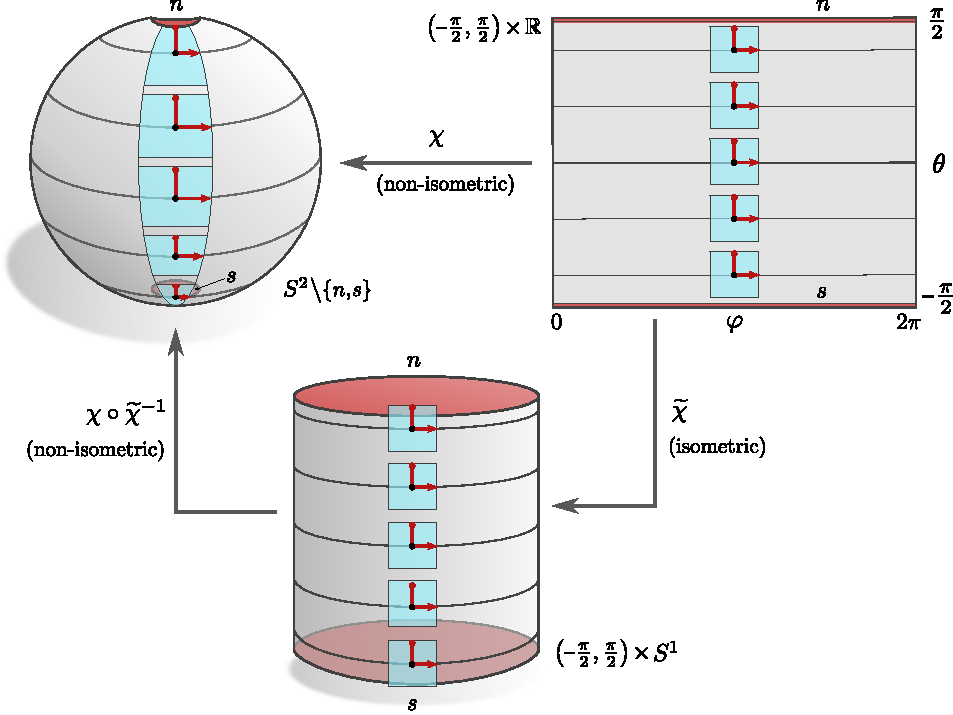
\includegraphics[width=.90\textwidth]{figures/G_structure_spherical_equirectangular_2.pdf}
    \caption{\small
        نگاشت مختصات کروی
        $\chi: \big(\protect\minus\frac{\pi}{2}, \frac{\pi}{2}\big) \times \R \to S^2 \backslash \{n,s\}$، معادله~\eqref{eq:spherical_coords}، زوایا $(\theta,\phi)$ را به نقاطی روی کره می‌فرستد.
        این نگاشت ایزومتریک نیست، که به این معنی است که پوش‌فوروارد چارچوب‌های راست‌هنجار
        $\big[ \frac{\partial}{\partial\theta}, \frac{\partial}{\partial\varphi} \big]$
        نسبت به \emph{متریک اقلیدسی} روی $\big(\protect\minus\frac{\pi}{2}, \frac{\pi}{2}\big) \times \R$ چارچوب‌هایی را که نسبت به \emph{متریک کروی} راست‌هنجار باشند، به دست نمی‌دهد.
        بنابراین یک کانولوشن اقلیدسی متعارف در مختصات $\big(\protect\minus\frac{\pi}{2}, \frac{\pi}{2}\big) \times \R$ متناظر با یک کانولوشن کروی نیست -- کرنل‌های آن با یک ضریب $\cos(\theta)$ در جهت طولی منقبض می‌شوند.
        از آنجا که فاصله‌ها بر حسب زوایا اندازه‌گیری می‌شوند، این عملیات بیشتر متناظر با یک کانولوشن روی یک استوانه است، که از طریق نگاشت ایزومتریک
        $\widetilde{\chi}: \big( {\textstyle \protect\minus\frac{\pi}{2}, \frac{\pi}{2}} \big) \times \R
        \to \big( {\textstyle \protect\minus\frac{\pi}{2}, \frac{\pi}{2}} \big) \times S^1$
        (معادله~\eqref{eq:cylindrical_coords}) در $\R^3$ جایگذاری شده است.
        یک کانولوشن کروی به $\{e\}$-ساختار نشان داده شده در شکل~\ref{fig:spherical_equirectangular_1} نیاز دارد.
    }
    \label{fig:spherical_equirectangular_2}
\end{figure}


با توجه به یک میدان ویژگی کروی در تصویر هم‌مستطیلی، ممکن است
علاوه بر این
وسوسه شویم که آن را مستقیماً با یک \lr{CNN} اقلیدسی متعارف پردازش کنیم و از تصویر کرنل از فضاهای مماس صرف نظر کنیم، همانطور که به عنوان مثال در~\cite{lai2017semantic,hu2017spherical} انجام شده است.
همانطور که در بخش~\ref{sec:instantiations_euclidean} بحث شد، چنین کانولوشن‌های اقلیدسی متناظر با کانولوشن‌های $\GM$ روی $\{e\}$-ساختار کانونی از $\big(\minus\frac{\pi}{2}, \frac{\pi}{2}\big) \times \R \subset \R^2$ هستند، که در شکل‌های~\ref{fig:G_structure_R2_1} و~\ref{fig:spherical_equirectangular_2} (بالا سمت راست) به تصویر کشیده شده است.
این $\{e\}$-ساختار از چارچوب‌های 
$\big[ \frac{\partial}{\partial\theta} ,\, \frac{\partial}{\partial\varphi} \big]$
تشکیل شده است، که نسبت به \emph{متریک اقلیدسی} از $\big(\minus\frac{\pi}{2}, \frac{\pi}{2}\big) \times \R$ راست‌هنجار هستند.
این چارچوب‌ها، با این حال، نسبت به \emph{متریک کروی} (معادله~\eqref{eq:spherical_embedding_metric_explicit}) راست‌هنجار نیستند، که در شکل~\ref{fig:spherical_equirectangular_2} (بالا سمت چپ) در انقباض چارچوب با ضریب $\cos(\theta)$ در جهت طولی منعکس شده است.
بنابراین یک کانولوشن $\GM$ روی این $\{e\}$-ساختار از نظر هندسی متناظر با یک کانولوشن کروی \emph{نیست}.
این بیشتر متناظر با یک کانولوشن $\GM$ روی یک استوانه است، که از طریق نگاشت مختصاتی \emph{ایزومتریک}
\begin{align}\label{eq:cylindrical_coords}
    \widetilde{\chi}:\, \big( {\textstyle \minus\frac{\pi}{2}, \frac{\pi}{2}} \big) \!\times \R
    \,\to\, \big( {\textstyle \minus\frac{\pi}{2}, \frac{\pi}{2}} \big) \!\times S^1,
    \quad (\theta,\phi) \mapsto
    \begin{pmatrix}
        \cos{\phi} \\
        \sin{\phi} \\
        \theta
    \end{pmatrix}
\end{align}
در $\R^3$ جایگذاری شده است.
در مقابل، $\{e\}$-ساختار نشان داده شده در شکل‌های~\ref{fig:G_structure_S2_2} و~\ref{fig:spherical_equirectangular_1} از چارچوب‌های
$\big[ \frac{\partial}{\partial\theta} ,\; \frac{1}{\cos(\theta)} \frac{\partial}{\partial\varphi} \big]$
تشکیل شده است، که نسبت به متریک کروی راست‌هنجار هستند.
توجه داشته باشید که این چارچوب‌ها و متریک کروی با ضریب $1/\cos(\theta)$ نسبت به همتایان اقلیدسی کانونی خود روی $\big( {\textstyle \minus\frac{\pi}{2}, \frac{\pi}{2}} \big) \times \R$ کشیده شده‌اند.


\citet{jiang2019spherical} یک رویکرد جایگزین برای کانولوشن‌های کروی روی $\{e\}$-ساختار نشان داده شده در شکل‌های~\ref{fig:G_structure_S2_2} و~\ref{fig:spherical_equirectangular_1} پیشنهاد می‌کنند.
به جای تعریف کرنل‌ها روی فضاهای مماس، آنها سیگنال را از طریق عملگرهای دیفرانسیل جزئی مرتبه دوم به شکل $w_{\id} + w_{e^A_1} \partial_1 + w_{e^A_2} \partial_2 + w_\textup{Laplace} (\partial_1^2 + \partial_2^2)$ پردازش می‌کنند، که در آن $\partial_i$ مشتق جزئی در جهت محور $i$-ام چارچوب را نشان می‌دهد و وزن‌های $w_{(\cdot)} \in \R^{\cout\times\cin}$ در طول آموزش بهینه‌سازی می‌شوند.
اینکه وزن‌ها مستقل از موقعیت هستند، متناظر با اشتراک وزن فضایی ما است.
این به همراه ناوردایی $\SO2$ از $\{e\}$-ساختار، که عملگرهای دیفرانسیل در امتداد آن تراز شده‌اند، هموردایی $\SO2$ عملیات را تضمین می‌کند.
در نظریه پیوسته، این مدل متناظر با یک کانولوشن $\GM$ در حد کرنل‌های بی‌نهایت کوچک است.
در عمل، \citet{jiang2019spherical} میدان ویژگی را روی یک مش ایکوسفر نمونه‌برداری می‌کنند و عملگرهای دیفرانسیل را بر حسب استنسیل‌های گسترده فضایی روی رئوس مش نمایش می‌دهند.
این کار، روش را معادل یک کانولوشن $\GM$ با کرنل‌های گسترده فضایی می‌کند.


مدل \citet{lee2019spherephd} دوباره روی یک ایکوسفر عمل می‌کند، با این حال، با یک $\{e\}$-ساختار به شدت تغییر یافته (ناهموار):
به جای تراز کردن چارچوب‌های مرجع به طوری که همگی به سمت قطب شمال اشاره کنند، چارچوب‌ها به طور متناوب به سمت شمال یا جنوب اشاره می‌کنند.
این طراحی از پیکسل‌بندی ایکوسفر، که وجوه مثلثی آن یا رو به شمال یا رو به جنوب هستند، الهام گرفته شده است.
بنابراین پیکسل‌های مجاور را می‌توان با کرنل‌هایی که نسبت به یکدیگر $180^\circ$ چرخانده شده‌اند، پردازش کرد.
نویسندگان استدلال می‌کنند که فرآیند آموزش باید این دوران را با یادگیری کرنل‌های راهبری‌پذیر متناسب جبران کند.
علی‌رغم دوران‌های شدید کرنل، $\{e\}$-ساختار تحت آن دسته از دوران‌های سمتی که چارچوب‌های رو به شمال را روی خودشان نگاشت می‌دهند، ناوردا است، که منجر به یک هموردایی تقریبی $\SO2$ کانولوشن می‌شود.


مدل‌های مورد بحث در این بخش به راحتی به دیگر اجسام دورانی ($\SO2$-ناوردا) مانند استوانه از شکل~\ref{fig:spherical_equirectangular_2} یا تخم‌مرغ از شکل~\ref{fig:isom_egg_main} تعمیم داده می‌شوند.
آنها علاوه بر این برای $\O2$-هموردا بودن، هنگام در نظر گرفتن یک ارتقا از $\{e\}$-ساختارها به $\Flip$-ساختارها، که متناظر با استفاده از کرنل‌های $\Flip$-راهبری‌پذیر است، همانطور که در شکل~\ref{fig:isom_invariant_kernel_field_quotient} نشان داده شده، تطبیق داده می‌شوند.